L'algorithme d'Angluin permet l'apprentissage actif d'automates déterministes finis définis dans le chapitre \ref{adf}. Ceux-ci représentant un langage régulier, celui-ci est effectivement appris. C'est cet algorithme, adapté à la situation, qui se trouve au cœur de LeVer, objet de ce mémoire.

La section \ref{angluin:fonc} donne une description générale de l'algorithme et de son exécution. Celui-ci repose sur différents concepts tels que :
\begin{itemize}
  \item le table filling algorithm de la section \ref{angluin:tfa} (permettant notemment de tester l'équivalence entre deux automates et de les minimiser au besoin)
  \item la relation \rl de la section \ref{angluin:rl} (portant sur des mots d'un langage) elle-même utilisée par le théorème de Myhill-Nerode
  \item le théorème de Myhill-Nerode de la section \ref{angluin:nerode}
  \item la table d'observation de la section \ref{angluin:to}, utilisée pour stocker la progression de l'algorithme
  \item la fermeture et la cohérence définies dans la section \ref{angluin:ferm}
\end{itemize}

Finalement, l'algorithme est donné dans la section \ref{angluin:algo} et sa complexité et ses limites y sont discutées.

\section{Fonctionnement}\label{angluin:fonc}Soit un langage régulier $L$. L'algorithme d'Angluin\cite{Angluin87} est un algorithme d'apprentissage actif d'automate qui permet d'apprendre un automate $A$ représentant $L(A)=L$. Il prend la forme d'un couple professeur/élève où :
\begin{itemize}
	\item L'élève applique l'algorithme d'Angluin $L^*$ en temps que tel pour construire un automate représentant le langage cible. Pour cela, il s'aide d'une table d'observation (section \ref{angluin:to})
	\item Le professeur a accès au langage que l'élève veut apprendre.
\end{itemize}

De plus, ce professeur contient deux oracles :
\begin{itemize}
	\item L'oracle d'appartenance. Soit un mot $w$. Appartient-il à $L$ ?
	\item L'oracle d'équivalence. Soit un automate $A_O$. Représente-t-il $L$ ? Si non, fournir un contre-exemple $w$.
\end{itemize}

\begin{figure}[H]
	\centering
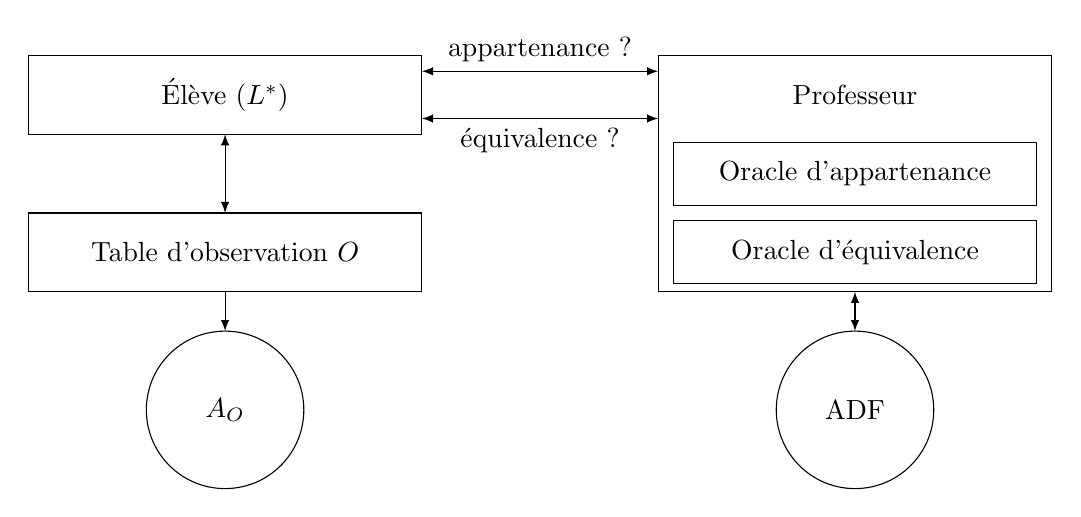
\begin{tikzpicture}
	\tikzset{>=latex}

	\draw (0,1) rectangle (5,0) node[pos=.5] {Élève ($L^*$)};
	\draw (8,1) rectangle (13,-2);

	\draw (8.2,-0.1) rectangle (12.8,-0.9) node[pos=.5] {Oracle d'appartenance};
	\draw (8.2,-1.1) rectangle (12.8,-1.9) node[pos=.5] {Oracle d'équivalence};

	\draw (0,-1) rectangle (5, -2) node[pos=.5] {Table d'observation $O$};

	\draw (10.5, -3.5) circle (1);
	\draw (2.5, -3.5) circle (1);

	\node[draw=none] at (10.5, 0.5) {Professeur} ;
	\node[draw=none] at (10.5,-3.5) {ADF};
	\node[draw=none] at (2.5,-3.5) {$A_O$};

	\draw[<->] (5,0.8) -- (8,0.8) node[pos=0.5,above] {appartenance ?};
	\draw[<->] (5,0.2) -- (8,0.2) node[pos=0.5,below] {équivalence ?};

	\draw[->] (2.5,-2) -- (2.5,-2.5);
	\draw[<->] (10.5, -2) -- (10.5,-2.5);
	\draw[<->] (2.5, 0) -- (2.5,-1);

\end{tikzpicture}
\caption{Vue schématique de l'algorithme d'Angluin}
\end{figure}

\begin{theorem}
	S'appuyant sur un professeur pour un langage régulier $L\subseteq\Sigma^*$, un élève peut utiliser l'algorithme d'Angluin $L^*$ pour apprendre l'ADF canonique $A$ représentant $L$ en un temps polynimial à $n$ le nombre d'états de $A$ et $m$ le nombre de contre-exemples reçus du professeur.
	Il effectue $\mathcal{O}(n)$ requêtes d'équivalence et $\mathcal{O}(mn^2)$ requêtes d'appartenance.\cite{Angluin87}
\end{theorem}

\begin{corollary}
	Si les requêtes d'appartenance et d'équivalence se font en temps polynomial en la taille de $A$, $L^*$ est en temps polynomial.
\end{corollary}

Attention cependant : cet algorithme part du postulat que le langage étudié est régulier.

Les prochaines section introduisent les différentes notions notemment necéssaires à la compréhension du fonctionnement de la table d'observation.

\section{Table Filling Algorithm}\label{angluin:tfa}
% ██████  ███████
% ██   ██ ██
% ██████  █████
% ██   ██ ██
% ██   ██ ███████



\subsection{Relation \re}\label{ss:re}

Soit un automate \automaton. Définissons la relation \re entre deux états :
$$xR_Ey \iff (\forall w \in \Sigma^*,\hdelta(x,w) \in F \iff \hdelta(y,w) \in F)$$

Intuitivement, ces deux états sont en relation si tout mot lu à partir de celui-ci mène à des états étant simultanément acceptants ou non.

\begin{proposition}[\re]
 \re est une relation d'équivalence.
\end{proposition}

\begin{proof}[\re est une relation d'équivalence] Montrer que \re est une relation d'équivalence revient à montrer qu'elle est réflexive, transitive et symétrique.
 \begin{itemize}
	 \item \textbf{Réflexive :} Soient un état $x \in Q_M$ et $w \in \Sigma^*$. Alors, $\hat{\delta}(x,w) \in F \iff \hat{\delta}(x,w) \in F$ et par définition, $xR_Ex$.
	 \item \textbf{Transitive :} Soient les états $x,y,z \in Q_M$ tels que $xR_Ey$ et $yR_Ez$ ainsi que $w \in \Sigma^*$. Par hypothèse, $\hat{\delta}(x,w) \in F \iff \hat{\delta}(y,w)\in F$ et $\hat{\delta}(y,w) \in F\iff \hat{\delta}(z,w) \in F$. Par transitivité de l'implication, on obtient $\hat{\delta}(x,w) \in F \iff \hat{\delta}(z,w)\in F$. On a donc $xR_Ez$.
	 \item \textbf{Symétrique : } Soient les états $x,y \in Q_M$ tels que $xR_Ey$ et un mot $w \in \Sigma^*$. Par hypothèse, $\hat{\delta}(x, w)\in F \iff \hat{\delta}(y, w)\in F$. En lisant la double implication depuis la droite, on a bien $\hat{\delta}(y, w) \in F\iff \hat{\delta}(x, w)\in F$ et donc $yR_Ex$.
 \end{itemize}
 \hfill$\square$
\end{proof}

\begin{corollary}
 \re sépare les états de $Q$ en classes d'équivalence.
\end{corollary}

La classe d'équivalence de tous les états en relation \re avec $q$ (qui sert alors de \emph{représentant}) se note $[[q]]$ ou par une lettre majuscule, typiquement $S$ ou $T$.

La \emph{congruence à droite} d'une relation $R$ entre des mots sur un alphabet $\Sigma$ est définie comme :
$$
\forall x,y \in \Sigma^*, xRy \Rightarrow \forall a \in \Sigma, xaRya
$$

\begin{proposition}[Congruence de \re]
 \re est congruente à droite.
\end{proposition}

\begin{proof}[Congruence de \re]\label{proof:rmcongruency}
 Si la relation est vraie pour deux état, elle reste valable pour les états atteints par la lecture d'un symbole quelconque. Soient les états $x,y \in Q_M$ tels que $xR_Ey$. Soit un symbole $a \in \Sigma$. Par hypothèse,
 $$\forall w \in \Sigma^*, \hat{\delta}(x, w) \in F \iff \hat{\delta}(y, w) \in F$$
 C'est donc vrai en particulier pour $w = au, u \in \Sigma*$. Dès lors,
 $$\hat{\delta}(x, au) \in F\iff \hat{\delta}(y, au)\in F$$
 $$\hat{\delta}(\delta(x,a),u) \in F\iff\hat{\delta}(\delta(y,a),u)\in F$$
 $$\hat{\delta}(p,u) \in F\iff \hat{\delta}(q,u)\in F$$

\hfill$\square$
\end{proof}

\begin{corollary}\label{col:st}
 Pour chaque symbole, toutes les transitions sortant d'une classe d'équivalence mènent à une même classe d'équivalence :
 $\forall a \in \Sigma, \exists T, \forall q \in S, \delta(q,a)\in T$ avec $T$ une classe d'équivalence.
\end{corollary}


% ████████ ███████  █████
%    ██    ██      ██   ██
%    ██    █████   ███████
%    ██    ██      ██   ██
%    ██    ██      ██   ██

\subsection{Table Filling Algorithm}
Certains états d'un automate peuvent être \emph{équivalents} selon la relation \re. Celui-ci peut alors être simplifié. Une façon de détecter ces équivalences est de construire un tableau via l'\emph{algorithme de remplissage de tableau}.

Celui-ci détecte les paires \emph{différenciables}, récursivement sur un automate \automaton. Un paire $\{p,q\}$ est différenciable s'il existe un mot $w$ tel qu'un chemin $\hdelta(p,w)$ mène à un état acceptant et $\hdelta(q,w)$ mène à un état non-acceptant ou vice-versa. $w$ sert alors de \emph{mot témoin}.

\textbf{Cas de base :} Si $p$ est un état acceptant et que $q$ ne l'est pas, alors la paire $\{p,q\}$ est différenciable. Le mot témoin est $\epsilon$.

\textbf{Pas de récurrence : } Soient $p,q$ des états de $Q$ et un symbole $a \in \Sigma$ tel que $\delta(p,a)=r$ et $\delta(q,a)=s$. Si $r$ et $s$ sont différenciables, alors $p$ et $q$ le sont aussi. En effet, il existe un mot \emph{témoin} $w$ qui permet de différencier $r$ et $s$. Alors le mot $aw$ est le mot témoin qui permet de différencier $p$ et $q$.

\begin{theorem}[Table d'équivalence]
 Si deux états ne sont pas distingués par l'algorithme de remplissage de tableau, les états sont équivalents (ils respectent la relation \re).
\end{theorem}

\begin{proof}

Considérons un automate déterministe fini quelconque \automaton. Supposons par l'absurde qu'il existe une paire d'états $\{p,q\}$ tels que :
\begin{enumerate}
	 \item $p$ et $q$ ne sont pas distingués par l'algorithme de remplissage de table.
	 \item Les états ne sont pas équivalents, $\not pR_E q$. Par extension, il existe un mot témoin $w$ différenciant $p$ et $q$.
\end{enumerate}

Une telle paire est une \emph{mauvaise paire}. Si il y a des mauvaises paires, chacune distinguée par un mot témoin, il doit exister un paire distinguée par le mot témoin le plus court. Posons $\{p,q\}$ comme étant cette paire et $w=a_1a_2\dots a_n$ le mot témoin le plus court qui les distingue. Dès lors, soit $\hdelta(p,w)$ est acceptant, soit $\hdelta(q,w)$ l'est, mais pas les deux.

Ce mot $w$ ne peut pas être $\epsilon$. Auquel cas, la table aurait été remplie dès l'étape d'induction de l'algorithme. La paire $\{p,q\}$ ne serait pas une mauvaise paire, ne respectant pas l'hypothèse 1.

$w$ n'étant pas $\epsilon$, $ |w| \ge 1$. Considérons les états $r = \delta(p,a_1)$ et $s=\delta(q,a_1)$. Ces états sont différenciés par $a_2a_3\dots a_n$ car $\hdelta(p,w) = \hdelta(r, a_2a_3\dots a_n)$ et $\hdelta(q,w) = \hdelta(s, a_2a_3\dots a_n)$ et $p$ et $q$ sont différenciables.

Cela signifie qu'il existe un mot plus petit que $w$ qui différencie deux états: le mot $a_2a_3\dots a_n$. Comme on a supposé que $w$ est le mot le plus petit qui différencie une mauvaise paire, $r$ et $s$ ne peuvent pas être une mauvaise paire. Donc, l'algorithme a du découvrir qu'ils sont différenciables.

Cependant, le pas de récurrence impose que $\delta(p, a_1)$ et $\delta(q, a_1)$ mènent à deux états différentiables implique que $p$ et $q$ le sont aussi. On a une contradiction de notre hypothèse : $\{p,q\}$ n'est pas une mauvaise paire.

Ainsi, s'il n'existe pas de mauvaise paire, c'est que chaque paire différenciable est reconnue par l'algorithme.

\hfill$\square$
\end{proof}

\begin{example}[Table d'équivalence] Voici une application de cet algorithme sur l'automate $A_2$, version réduite de l'automate $A_1$ de la figure \ref{fig:a1}.

\begin{figure}[H]
 \centering
 \begin{tikzpicture}[->,>=stealth',shorten >=1pt,auto,node distance=3cm, semithick, bend angle=10]

 \tikzstyle{every state}=[circle]

 \node[initial,state] (A)                    {$q_0$};
 \node[state]         (B) [below right of=A] {$q_1$};
 \node[state]         (C) [below left of=A] {$q_2$};
 \node[accepting,state]         (D) [below right of=B] {$q_3$};
 \node[state]         (E) [below left of=C]       {$q_4$};
 \node[state]         (F) [below right of=C]       {$q_5$};

 \path 	(A) 	edge              node {a} (C)
 edge              node {b} (B)
 (B) 	edge              node {a} (D)
 edge [bend left]  node {b} (F)
 (C) 	edge              node {a} (E)
 edge              node {b} (F)
 (D) 	edge [loop above] node {a,b} (D)
 (E) 	edge [loop above] node {a,b} (E)
 (F) 	edge              node {a} (D)
 edge [bend left]  node {b} (B);
 \end{tikzpicture}
 \caption{Automate $A_2$}\label{fig:a2}
\end{figure}

La première étape est de remplir la table avec l'algorithme précédant. Tout état est distinguable de $q_3$ : il est le seul état acceptant. 5 cases peuvent déjà êtres cochées. Le reste de la table est remplie par induction.

\begin{figure}[H]
 \centering
 \begin{tabular}{ccccccc}
	 \cline{2-2}
	 \multicolumn{1}{c|}{$q_1$} & \multicolumn{1}{c|}{x} &&&&\\
	 \cline{2-3}
	 \multicolumn{1}{c|}{$q_2$} & \multicolumn{1}{c|}{x} &\multicolumn{1}{c|}{x}&&&\\
	 \cline{2-4}
	 \multicolumn{1}{c|}{$q_3$} & \multicolumn{1}{c|}{x} &\multicolumn{1}{c|}{x}&\multicolumn{1}{c|}{x}&&\\
	 \cline{2-5}
	 \multicolumn{1}{c|}{$q_4$} & \multicolumn{1}{c|}{x} &\multicolumn{1}{c|}{x}&\multicolumn{1}{c|}{x}&\multicolumn{1}{c|}{x}&\\
	 \cline{2-6}
	 \multicolumn{1}{c|}{$q_5$} & \multicolumn{1}{c|}{x} & \multicolumn{1}{c|}{}&\multicolumn{1}{c|}{x}&\multicolumn{1}{c|}{x}&\multicolumn{1}{c|}{x}\\
	 \cline{2-6}
	 \multicolumn{1}{c}{} & $q_0$&$q_1$&$q_2$&$q_3$&$q_4$\\

 \end{tabular}
 \caption{Table filling pour $A_2$, décelant des équivalences d'états}
 \label{fig:ta2}
\end{figure}
\end{example}
\stepcounter{algo}
\begin{complexity}

Considérons $n$ le nombre d'états d'un automate, et $k$ la taille de l'alphabet $\Sigma$ supporté.

Si il y a $n$ états, il y a $\begin{pmatrix}n\\2\end{pmatrix}$ soit $\frac{n(n-1)}{2}$ paires d'états. A chaque itération (sur l'ensemble de la table), il faut considérer chaque paire, et vérifier si un de leur successeurs est différentiable. Cette étape prend au plus $\mathcal{O}(k)$ pour tester chaque successeurs potentiel (en fonction du symbole lu).  Ainsi, une itération sur la table se fait en $\mathcal{O}(kn^2)$. Si une itération ne découvre pas de nouveaux état différentiable s'arrête. Comme la table a une taille en $\mathcal{O}(n^2)$ et qu'à chaque étape un élément au minimum doit y être coché, la complexité totale de l'algorithme est en $\mathcal{O}(kn^4)$.

Cependant, il existe des pistes d'amélioration. La première est d'avoir, pour chaque paire $\{r,s\}$ une liste des paire $\{p,q\}$ qui, pour un même symbole, mènent à $\{r,s\}$. On dit de ces paires qu'elles sont dépendantes. Si la paire $\{r,s\}$ est marquée comme différenciable, leurs paires dépendantes seront de facto différenciables.

Cette liste peut être construite en considérant chaque symbole $a \in \Sigma$ et ajoutant les paires $\{p,q\}$ à chacune de leur dépendance $\{\delta(p,a),\delta(q,a)\}$. Cette étape prend au plus $k.\mathcal{O}(n^2)=\mathcal{O}(kn^2)$. (Le nombre de symboles multiplié par le nombre de paires à considérer).

Ensuite, il suffit de partir des cas initiaux (se reposant sur le cas de base de l'algorithme), et de marquer tous leurs états dépendants comme différentiables, tout en ajoutant leur propre liste à chaque fois. La complexité de cette exploration est bornée par le nombre d'éléments dans une liste et le nombre de listes. Respectivement, $k$ et $\mathcal{O}(n^2)$, ce qui donne $\mathcal{O}(kn^2)$ pour cette exploration.

La complexité totale revient à $\mathcal{O}(kn^2)$.
\end{complexity}


% ███    ███ ██ ███    ██ ██ ███    ███
% ████  ████ ██ ████   ██ ██ ████  ████
% ██ ████ ██ ██ ██ ██  ██ ██ ██ ████ ██
% ██  ██  ██ ██ ██  ██ ██ ██ ██  ██  ██
% ██      ██ ██ ██   ████ ██ ██      ██

\subsection{Minimisation}
La minimisation d'automate se fait en deux étapes :
\begin{enumerate}
 \item Se débarrasser de tous les états injoignables : ils ne participent pas à la construction du langage représenté
 \item Grâce aux équivalences d'états trouvées grâce à l'algorithme de remplissage de tableau défini au point \ref{ss:tfa}, construire un nouvel automate.
\end{enumerate}

Soit un automate déterministe fini \automaton. Les états non-atteignables peuvent être supprimés de $Q$ et de $\delta$.

Pour minimiser cet automate, il faut :
\begin{enumerate}
 \item Générer la table de différenciation.
 \item Séparer $Q$ en classes d'équivalences
 \item Construire l'automate canonique $C=(Q_C,\Sigma, \delta_C, q_C, F_C)$:
 \begin{itemize}
	 \item Soit $S$ une des classes d'équivalence obtenues par la table de différenciation.
	 \item Ajouter $S$ à $Q_C$ et à $F_C$ si $S$ contient un état acceptant : $q\in S, q\in F$.
	 \item Si $S$ contient $q_0$ l'état initial de $A$, alors $S$ est $q_C$ l'état initial de $C$.
	 \item Pour un symbole $a \in \Sigma$, alors il doit exister une classe d'équivalence $T$ tel que pour chaque état $\forall q \in S,\delta(q,a) \in T$. Si ce n'est pas le cas, c'est que deux états $p$ et $q$ dans $S$ mènent à différentes classes d'équivalences. Or, ces deux états sont différenciables, et ne pourraient pas appartenir tous deux à $S$ par construction. Ce fait est déjà mentionné dans le corollaire \ref{col:st}. On peut écrire $\delta_C(S,a)=T$. Pour rappel, la fonction $\delta$ est définie pour tout état et tout symbole. Rien n'empêche $T=S$.
 \end{itemize}
\end{enumerate}


\begin{example}

 Considérons l'automate $A_1$ représenté à la figure \ref{fig:a1}. En supprimant l'état $q_6$ qui n'est pas atteignable, on obtient l'automate $A_2$ de la figure \ref{fig:a2}.

 Le tableau de la figure \ref{fig:ta2} sert d'exemple pour l'algorithme de remplissage de tableau, sur $A_2$.
 $A_3$.

 En appliquant l'algorithme, qui peut se résumer intuitivement à fusionner les états équivalents, on obtient l'automate $A_3$ de la figure \ref{fig:a3}.

 \begin{figure}[H]
	 \centering
	 \begin{tikzpicture}[->,>=stealth',shorten >=1pt,auto,node distance=3cm, semithick, bend angle=10]

	 \tikzstyle{every state}=[circle]

	 \node[initial,state] (A)                    {$q_0$};
	 \node[state]         (B) [below right of=A] {$q_1$};
	 \node[state]         (C) [below left of=A] {$q_2$};
	 \node[accepting, state]         (D) [below right of=B] {$q_3$};
	 \node[state]         (E) [below left of=C]       {$q_4$};

	 \path
	 (A) 	edge              node {a} (C)
	 edge              node {b} (B)
	 (B) 	edge              node {a} (D)
	 edge [loop above] node {b} (B)
	 (C) 	edge              node {a} (E)
	 edge              node {b} (B)
	 (D) 	edge [loop above] node {a,b} (D)
	 (E) 	edge [loop above] node {a,b} (E);
	 \end{tikzpicture}
	 \caption{Automate $A_3$}\label{fig:a3}
 \end{figure}

 Une expression régulière ($(b+ab)b^*a(a+b)^*$) peut être déduite pour $L$ grâce à cet automate. Cette expression régulière est celle de l'exemple \ref{ex:regex}
\end{example}


\begin{theorem}[Minimalité de l'automate réduit]
 Soit un ADF $A$ et soit $C$ l'automate construit par cet algorithme de minimisation. Aucun automate équivalent à $A$ n'a moins d'états que $C$. De plus, chaque automate ayant autant d'états que $C$ peut être transformé en celui-ci par homomorphisme.
\end{theorem}


\begin{proof}
 Prouvons que l'algorithme de minimisation fourni un automate minimum (il n'en existe aucun comportant moins d'états pour un même langage)
 Soient un ADF $A$ et $C$ l'automate obtenu par l'algorithme de minimisation. Posons que $C$ comporte $k$ états.

 Par l'absurde, supposons qu'il existe $M$ un ADF minimisé équivalent à $A$ mais comptant moins d'états que $C$. Posons qu'il en comporte $l<k$.
 Appliquons l'algorithme de remplissage de table sur $C$ et $M$, comme s'ils étaient un seul ADF, comme proposé dans la section \ref{ss:eqauto}. Les états initiaux sont équivalents (pas différentiables) puisque $L(C)=L(M)$. Dès lors, les successeurs pour chaque symboles sont eux aussi équivalent. Le cas contraire impliquerait que états initiaux sont différentiables, ce qui n'est pas le cas.
 De plus, ni $C$ ni $M$ n'ont un état inaccessible, sinon il pourrait être éliminé, résultant en un automate comportant moins d'états pour un même langage.
 Soit $p$ un état de $C$. Soit un mot $a_1a_2\dots a_i$, qui mène de l'état initial de $C$ à $p$. Alors, il existe un état $q$ de $M$ équivalent à $p$. Puisque les états initiaux sont équivalents, et que par induction, les états obtenus par la lecture d'un symbole le sont aussi, l'état $q$ dans $M$ obtenu par la lecture du mot $a_1a_2\dots a_i$ est équivalent à $p$. Ceci signifie que tout état de $C$ est équivalent à au moins un état de $M$.
 Or, $lk>l$. Cela signifie qu'il doit exister au moins deux états de $C$ équivalents à un même état de $M$ et donc équivalent entre eux. Il y a la contradiction : par construction, les états de $C$ sont tous différentiables les uns des autres. La supposition de l'existence de $M$ est fausse. Il n'existe pas d'automate équivalent à $A$ comportant moins d'états que $C$.

 \hfill$\square$
\end{proof}

\begin{proof}
 Prouvons que tout automate minimal pour un langage est $C$, à un isomorphisme sur les noms des états près.

 Soit $A$ un ADF pour un langage $L$. Soient $C$ un ADF obtenu par l'algorithme de minimisation et $M$ un automate minimal comportant autant d'états que $C$.

 Comme mentionné dans la preuve précédente, il doit y avoir une équivalence 1 à 1 entre chaque état de $C$ et de $M$. (Au minimum 1 et au plus 1). De plus, aucun état de $M$ ne peut être équivalent à 2 états de $C$, selon le même argument.

 Dès lors, l'automate minimisé, dit \emph{canonique} est unique à l'exception du renommage des différents états.

 \hfill$\square$
\end{proof}


% ███████  ██████  ██    ██ ██ ██    ██
% ██      ██    ██ ██    ██ ██ ██    ██
% █████   ██    ██ ██    ██ ██ ██    ██
% ██      ██ ▄▄ ██ ██    ██ ██  ██  ██
% ███████  ██████   ██████  ██   ████
%             ▀▀


\subsection{Appartenance et équivalence}
Considérons les automates $A_H$ et $A_I$ donnés dans les figures \ref{fig:ah} et \ref{fig:ai}

\begin{minipage}{0.4\linewidth}
 \begin{figure}[H]
	 \centering
	 \begin{tikzpicture}[->,>=stealth',shorten >=1pt,auto,node distance=2cm and 5cm, semithick, bend angle=10]

	 \tikzstyle{every state}=[circle]

	 \node[initial,state]	(A)					{$q_0$};
	 \node[state]			(B)	[right= of A]	{$q_1$};
	 \node[accepting,state]	(C) [below of=A]	{$q_2$};
	 \node[accepting,state]	(D)	[below of=B]	{$q_3$};
	 \node[accepting,state]	(E)	[below of=C]	{$q_4$};
	 \node[state]			(F)	[below of=D]	{$q_5$};

	 \path
	 (A)	edge	[bend left]		node{a}		(B)
	 (A)	edge					node{b}		(C)
	 (B) edge	[bend left]		node{a}		(A)
	 (B) edge					node{b}		(D)
	 (C)	edge					node{a}		(E)
	 (C)	edge					node[near start]{b}		(F)
	 (D)	edge					node[near start, above]{a}		(E)
	 (D)	edge					node{b}		(F)
	 (E)	edge	[loop below]	node{a}	(E)
	 (E) edge					node{b} (F)
	 (F)	edge	[loop below]	node{a,b}	(F)

	 ;
	 \end{tikzpicture}
	 \caption{Automate $A_H$, du livre d'Hopcraft et al. de 1979\cite{Hopcroft79} (Fig3.2)}\label{fig:ah}
 \end{figure}
\end{minipage}\hspace{0.2\linewidth}
\begin{minipage}{0.4\linewidth}
 \begin{figure}[H]
	 \centering
	 \begin{tikzpicture}[->,>=stealth',shorten >=1pt,auto,node distance=1cm and 1cm, semithick, bend angle=10]

	 \tikzstyle{every state}=[circle]

	 \node[initial,state]	(A)					{$q_6$};
	 \node[accepting,state]	(B)	[right= of A]	{$q_7$};
	 \node[state]			(C) [right= of B]	{$q_8$};

	 \path
	 (A)	edge					node{b}		(B)
	 (A)	edge	[loop above]	node{a}		(A)
	 (B) edge					node{b}		(C)
	 (B) edge	[loop above]	node{a}		(B)
	 (C)	edge	[loop above]	node{a,b}	(C)

	 ;
	 \end{tikzpicture}
	 \caption{Automate $A_I$, provenant également de \cite{Hopcroft79}. Les états ont été renommés. }\label{fig:ai}
 \end{figure}
\end{minipage}

Il est possible de remplir un tableau via l'algorithme éponyme. Pour ce faire, les deux automates sont considérés comme un seul dont les états sont disjoints.

\begin{figure}[H]
 \centering
 \begin{tabular}{ccccccccc}
	 \cline{2-2}
	 \multicolumn{1}{c|}{$q_1$}&\multicolumn{1}{c|}{} &&&&&&&\\
	 \cline{2-3}
	 \multicolumn{1}{c|}{$q_2$}&\multicolumn{1}{c|}{x} &\multicolumn{1}{c|}{x}&&&&&&\\
	 \cline{2-4}
	 \multicolumn{1}{c|}{$q_3$}&\multicolumn{1}{c|}{x}&\multicolumn{1}{c|}{x}&\multicolumn{1}{c|}{}&&&&&\\
	 \cline{2-5}
	 \multicolumn{1}{c|}{$q_4$}&\multicolumn{1}{c|}{x}&\multicolumn{1}{c|}{x}&\multicolumn{1}{c|}{}&\multicolumn{1}{c|}{}&&&&\\
	 \cline{2-6}
	 \multicolumn{1}{c|}{$q_5$}&\multicolumn{1}{c|}{x}&\multicolumn{1}{c|}{x}&\multicolumn{1}{c|}{x}&\multicolumn{1}{c|}{x}&\multicolumn{1}{c|}{x}&&&\\
	 \cline{2-7}
	 \multicolumn{1}{c|}{$q_6$}&\multicolumn{1}{c|}{}&\multicolumn{1}{c|}{}&\multicolumn{1}{c|}{x}&\multicolumn{1}{c|}{x}&\multicolumn{1}{c|}{x}&\multicolumn{1}{c|}{x}&&\\
	 \cline{2-8}
	 \multicolumn{1}{c|}{$q_7$}&\multicolumn{1}{c|}{x}&\multicolumn{1}{c|}{x}&\multicolumn{1}{c|}{}&\multicolumn{1}{c|}{}&\multicolumn{1}{c|}{}&\multicolumn{1}{c|}{x}&\multicolumn{1}{c|}{x}&\\
	 \cline{2-9}
	 \multicolumn{1}{c|}{$q_8$}&\multicolumn{1}{c|}{x}&\multicolumn{1}{c|}{x}&\multicolumn{1}{c|}{x}&\multicolumn{1}{c|}{x}&\multicolumn{1}{c|}{x}&\multicolumn{1}{c|}{}&\multicolumn{1}{c|}{x}&\multicolumn{1}{c|}{x}\\
	 \cline{2-9}
	 \multicolumn{1}{c}{} & $q_0$& $q_1$ & $q_2$ & $q_3$ & $q_4$ & $q_5$ & $q_6$ & $q_7$\\

 \end{tabular}
 \caption{Tableau généré par l'application de l'algorithme sur $A_H$ et $A_I$}\label{fig:tahi}
\end{figure}

De cette table, toujours grâce aux conclusions précédentes, il est possible d'extraire des classes d'équivalences :
\begin{itemize}
 \item $C_0 = \{q_0, q_1, q_6\}$
 \item $C_1 = \{q_2, q_3, q_4, q_7\}$
 \item $C_2 = \{q_5, q_8\}$
\end{itemize}

En particulier, la classe $C_0$ souligne que les états initiaux sont équivalents. Cela signifie, par définition, que tout mot $w$ lu en partant d'un de ces états sera soit accepté dans les deux automates, soit refusé dans les deux. $A_H$ et $A_I$ définissent donc le même langage.
\stepcounter{algo}
\begin{complexity}
 Reposant sur la construction de la table d'équivalence d'états, la complexité est en $\mathcal{O}(kn^2)$, avec $k$ la taille de l'alphabet et $n$ le nombre d'états. L'étape supplémentaire, la lecture de cette table, est en temps constant et n'impacte pas la complexité.
\end{complexity}


Les différentes notions liées à l'égalité : les propriétés de réflexivité, transitivité et symétrie ont été démontrées dans la section \ref{ss:rm}.

\section{\rl}\label{angluin:rl}Soit un langage $L$ sur un alphabet $\Sigma$.

Soit la relation $R_L\subseteq\Sigma^*\times\Sigma^*$. Deux mots $x$ et $y$ respectent la \emph{relation de Myhill-Nérode $R_W$} si

$$\forall z \in \Sigma^*, xz \in L \Leftrightarrow yz \in L$$

Intuitivement, deux mots sont en relation si pour tout mot qu'on leur concatène, les deux mots résultants sont tous deux dans le langage $L$ ou non.

Cette relation est utilisée au fondement de l'algorithme d'Anluin pour séparer le langage en différentes classes, jusqu'à identifier celles qui sont acceptées de celles qui ne le sont pas.

\begin{lemma}
	Cette relation est une relation d'équivalence. De plus, elle est congruente à droite. C'est à dire que si $xR_Ly$, alors pour tout symbole $a \in \Sigma$, $xaR_Lya$
\end{lemma}

\begin{proof}[Equivalence et Congruence à droite]
	Dire d'une relation qu'elle décrit une équivalence, revient à dire qu'elle est réflexive, transitive et symétrique
\begin{itemize}
		\item\textbf{Réflexive :} Soit $x \in \Sigma^*$. Soit $z \in \Sigma^*$. Montrer que $xR_Lx$ est vrai revient à montrer que $ xz \in L \Leftrightarrow xz \in L$ est vrai. $R_L$ est donc réflexive.
		\item \textbf{Symétrique :} Soient $x, y \in \Sigma^*$ tels que $xR_Ly$. Soit $w \in \Sigma^*$. Montrer que $yR_Lx$ revient à montrer que $ yw \in L \Leftrightarrow xw \in L$. Or, par hypothèse, $ xz \in L \Leftrightarrow yz \in L$, qui peut s'écrire aussi $ yz \in L \Leftrightarrow xz \in L$ pour tout $z \in \Sigma^*$, et en particulier $z=w$.
		\item \textbf{Transitive :} Soient $x,y,u \in \Sigma^*$ tels que $xR_Ly$ et $yR_Lz$. Soit $w \in \Sigma^*$. Comme $ xz \in L \Leftrightarrow yz \in L$ et $ yz \in L \Leftrightarrow uz \in L$ pour tout $z \in \Sigma^*$ (par hypothèse), c'est vrai en particulier pour $z=w$. Dès lors,  $ xw \in L \Leftrightarrow yw \in L$ et $ yw \in L \Leftrightarrow uw \in L$. Par transitivité de l'implication, on obtient $ xw \in L \Leftrightarrow uw \in L$, à savoir $xR_Lu$.
	\end{itemize}

	$R_L$ est congruente à droite. Soient $x,y \in \Sigma^*$ tels que $xR_Ly$. Soit $a \in \Sigma$. Par hypothèse, $ xz \in L \Leftrightarrow yz \in L$ pour tout $z \in \Sigma^*$. Cela doit donc être vrai en particulier pour le mot $z=aw$ avec $w$ quelconque. En remplaçant dans l'hypothèse, on obtient  $ xaw \in L \Leftrightarrow yaw \in L$. Ce qui montre que $xaR_Lya$.

\hfill$\square$
\end{proof}

\section{Théorème de Myhill-Nérode}\label{angluin:nerode}

	Le thèorème de Myhill-Nérode est un résultat fort utilisant la relation \rl. Il permet de construire un automate à partir de celle-ci.

	Cependant, avant d'énoncer le théorème de Myhill-Nérode, il faut s'intéresser à la relation d'équivalence \ra, qui facilite l'écriture de la preuve. \rl s'intéresse directement au langage alors que \ra s'intéresse à un automate qui la représente.

	\begin{definition}[Relation \ra]
		Soit un automate \automaton. Soient deux mots $x,y\in\Sigma^*$. Alors la relation $xR_Ay$ est vraie si et seulement si $\hdelta(q_0,x)=\hdelta(q_0,y)$.
	\end{definition}

	Intuitivement, deux mots sont en relation \ra par rapport à un automate $A$ s'ils mènent à un même état dans celui-ci (ou à des états équivalents).

	\begin{lemma}
		\ra est une relation d'équivalence congruente à droite.
	\end{lemma}

	\begin{proof}
		Prouver qu'une relation est dite d'équivalence, il faut prouver que celle-ci est transitive, réflexive et symétrique.
		Soit un automate \automaton.
		\begin{itemize}
		\item \ra est transitive. Soient $x,y,z\in\Sigma^*$. Supposons que $xR_Ay$ et $yR_Az$. On a bien $\hdelta(q_0,x)=\hdelta(q_0,y)=\hdelta(q_0,z)$ par la transitivité de l'équivalence entre deux états.
		\item \ra est réflexive. Soit $y\in\Sigma^*$. On a bien $\hdelta(q_0,y)=\hdelta(q_0,y)$ par réflexiviré de l'équivalence sur un état.
		\item \ra est symétrique. Soient $x,y\in\Sigma^*$. Supposons que $xR_Ay$. On a bien $\hdelta(q_0,y)=\hdelta(q_0,x)$ par symétrie de l'équivalence entre deux états.
		\end{itemize}

		\ra est congruente à droite. Soient $x,y\in\Sigma^*$ tels que $xR_Ay$. Soit $z\in\Sigma^*$. Montrons que $xzR_Ayz$. $\hdelta(q_0,xz)=\hdelta(\hdelta(q_0,x),z)=\hdelta(\hdelta(q_0,y),z)=\hdelta(q_0,yz)$.

		\hfill$\square$
	\end{proof}

	\begin{theorem}
		Les trois énoncés suivants sont équivalents :
		\begin{enumerate}
			\item Un langage $L\subseteq\Sigma^*$ est accepté par un ADF.
			\item Il existe une congruence à droite sur $\Sigma^*$ d'index fini telle que $L$ est l'union de certaines classes d'équivalence.
			\item La relation d'équivalence $R_L$ est d'index fini.
		\end{enumerate}
	\end{theorem}


	\begin{proof}\label{proof:mn}
		La preuve d'équivalence se fait en prouvant chaque implication de façon cyclique :\\

		$(1)\rightarrow(2)$ Supposons que (1) soit vrai, c'est-à-dire que le langage $L$ est accepté par un automate déterministe \automaton. Considérons la relation d'équivalence congruente à droite \ra. Soit un mot $w\in\Sigma^*$. Alors tout mot $x\in\Sigma^*$ tel que $\hdelta(q_0,x)=\hdelta(q_0,w)$ appartient à la même classe d'équivalence $[w]$. Or, la fonction $\hdelta$ retourne un état $q\in Q$. Chaque classe d'équivalence sur $\Sigma$ correspond alors à un état de l'automate. Comme $Q$ est fini, \ra est d'index fini. De plus, un sous-ensemble des classes d'équivalences doit correspondre aux états acceptants $q\in F$. Alors, $L$ est l'union de ces classes d'équivalence.

		$(2)\rightarrow(3)$ Supposons qu'il existe une relation $E$ satisfaisant (2). Montrons que chaque classe de celle-ci est intégralement contenue dans une seule classe de \rl. Puisque $E$ est d'index fini, c'est un argument suffisant pour montrer que \rl est d'index fini. Soit $x,y$ tels que $xEy$. Comme $E$ est congruente à droite, pour tout mot $z \in \Sigma^*$, on sait que $xzEyz$. Comme $L$ est un union de ces classes d'équivalence, $xzEyz$ implique que $xz \in L \Leftrightarrow yz \in L$, ce qui revient à $xR_Ly$. Cela signifie que tout mot dans la classe d'équivalence de $x$ définie par $E$ se retrouve dans la même classe d'équivalence que $x$ cette fois définie par \rl. Ceci permet de conclure que chaque classe d'équivalence de $E$ est contenue dans une classe d'équivalence de \rl et donc que \rl est d'index fini.

		$(3)\rightarrow(1)$ Considérons la relation \rl définie précédemment. Soit un automate \automaton défini comme suit :
		\begin{itemize}
			\item Chaque état $q\in Q$ correspond à une classe d'équivalence de \rl.
			\item Comme \rl se défini pour un langage, l'alphabet $\Sigma$ de celui-ci est déjà défini.
			\item Si $[[\epsilon]]$ est la classe d'équivalence de $\epsilon$ sur \rl, $q_0$ correspond à cette classe.
			\item Si $q$ représente $[[x]]$ et $q_1$ représente $[[xa]]$, alors $\delta(q,a)=q_1$. Cette définition est cohérente car \rl est congruente à droite.
			\item $F = \{[[x]]|x \in L\}$.
		\end{itemize}
		Cet automate est déterministe par la définition de $\delta$ et fini car $Q$ l'est, le nombre de classes de \rl étant fini par hypothèse. De plus, cet automate accepte tout mot $x\in L$ puisque $\delta(q_0,x)=[[x]]\in F$(par définition, puisque $x\in L$).
		\hfill$\square$
	\end{proof}


	\begin{corollary}\label{col:constadf}
		La partie $(3)\rightarrow(1)$ de la preuve \ref{proof:mn} donne une méthode permettant de construire un ADF à partir des classes d'équivalences de la relation \rl.
	\end{corollary}

On peut prouver que l'automate obtenu de cette façon est l'automate minimal de $L$. Une preuve est disponible dans l'ouvrage \cite{Hopcroft79} en lien avec le théorème 3.10.

\section{Table d'observation}\label{angluin:to}
	Une \emph{table d'observation} est un tableau défini par $O=(R,S,T)$ avec $R\subseteq\Sigma^*$ un ensemble de mots \emph{représentants}, $S\subseteq\Sigma^*$ un ensmble de mots \emph{séparateurs} et $T:(R\bigcup R.\Sigma)\rightarrow\{0,1\}$ une fonction représentant le contenu de la table.\cite{Neider14}
	Soit un langage $L$ qui est en train d'être appris par l'algorithme d'Angluin. Soit un mot $w\in L$. Alors, $w$ appartient à une classe d'équivalence $[[u]]$ avec $u\in L$. Dans ce cas, $T(w)=1$. Au contraire, si $w\notin L$, alors $T(w)=0$.

	Pour une table d'observation $O$, deux mots $u,v$ peuvent être \emph{équivalents sur O}, c'est-à-dire $uR_Ov$. $u$ et $v$ sont équivalents sur $O$ si et seulement si $\forall w \in S, T(uw)=T(vw)$. Intuitivement, $uR_Ov$ si les lignes correspondant à leur classe d'équivalence ont la même séquence de $0$ et de $1$.

	\begin{proposition}
		Soient $u,v \in \Sigma^*$, un langage $L$ et une table d'observation $O$ associée à ce langage. Si $uR_Lv$, alors $uR_Ov$.
	\end{proposition}

	\begin{proof}
		Soient un langage $L$, $u,v \in \Sigma^*$ tels que $uR_Lv$ et une table d'observation $O$ associée à $L$.
		Comme $uR_Lv$, alors pour tout mot $w\in\Sigma^*$, $uw\in L \iff vw\in L$. C'est donc vrai en particulier pour tout $w\in S$. Dès lors, $\forall w \in S, T(uw)=T(vw)$.
		\hfill$\square$
	\end{proof}

	\begin{corollary}
		Le nombre de classes d'équivalence sur \ro est inférieur ou égal à celui de classes d'équivalence sur \rl.
	\end{corollary}

	Cette table $O$ représente la compréhension actuelle de l'élève du langage $L$. D'itération en itération, $R_O$ représente de mieux en mieux $R_L$ jusqu'à ce que l'automate induit de cette table soit jugé équivalent par le professeur. L'automate induit l'est par l'application du corollaire \ref{col:constadf}.

\section{Fermeture et cohérence}\label{angluin:ferm}Les propriété de fermeture (\ref{ss:ferm}) et de cohérence (\ref{ss:coh}) qui sont définies ici sont à respecter à chaque itération de l'algorithme d'Angluin.


\subsection{Fermeture}\label{ss:ferm}
La propriété de \emph{fermeture} s'exprime mathématiquement par

$$ \forall u \in R, \forall a \in \Sigma, \exists v \in R, ua R_O v$$

Cette propriété peut être vérifiée par cet algorithme, expliqué de façon visuelle sur la table O :

\begin{algorithm}[H]
	\begin{algorithmic}[1]
		\ENSURE si la fermeture est respectée ou non

		\FORALL {élément $w$ de la section $R$}
		\FORALL {symbole $a$ dans $\Sigma$}
			\IF {$wa$ est dans $R$}
				\STATE continuer
			\ELSE
				\STATE \COMMENT{$wa$ est dans $R.\Sigma$ par construction}
				\IF {La ligne de $wa$ dans $T$ est différente de celle de $w$}
					\RETURN Faux
				\ENDIF
			\ENDIF
		\ENDFOR
		\ENDFOR
		\RETURN Vrai
	\end{algorithmic}
	\caption{Vérification de la fermeture}\label{alg:fermeture}
\end{algorithm}

\subsection{Cohérence}\label{ss:coh}

La propriété de \emph{cohérence} se définit mathématiquement comme

$$ \forall u,v \in R, u R_O v \Rightarrow \forall a \in \Sigma, ua R_O va$$

Concrètement, il s'agit de prendre deux mots ($u,v$) dans $R$ ayant la même ligne dans $T$ et vérifier, pour chaque symbole ($a$), s'ils ($ua,va$) ont la même ligne dans $T$.

\begin{example}
	Soit la table d'observation O de la table \ref{tab:Oex} :

	\begin{table}[H]
		\centering
	\begin{tabular}{|c|c|c|}
		\hline
		$O$ & $\epsilon$ & a\\
		\hline
		$\epsilon$ & 0 & 0\\
		$a$ & 0 & 0\\
		\hline
		$aa$ & 0 & 1\\
		\hline
	\end{tabular}\caption{Table d'observation O}\label{tab:Oex}
\end{table}
	\vspace{0.5cm}
	Cette table n'est pas cohérente. En effet, $\epsilon R_O a$ mais en ajoutant le symbole $a\in \Sigma$, on obtient $\neg (a R_O aa)$. Les lignes ont les mêmes valeurs, mais les lignes obtenues par la concaténation du symbole $a$ ont des valeurs différentes.
\end{example}

\section{Algorithme et complexité}\label{angluin:algo}
Le pseudocode de l'algorithme d'Angluin est fourni par l'algorithme \ref{alg:angluin}\cite{Neider14}. Celui-ci repose sur les oracles du professeur et l'algorithme \ref{alg:corr}, remplissant les lignes de $T$ encore vides. Le code est suivi d'un exemple d'exécution.

\begin{algo}[Algorithme d'Angluin $L^*$]\label{alg:angluin}
  \begin{algorithmic}[1]
    \REQUIRE Un professeur pour le langage régulier $L\subseteq\Sigma^*$
		\ENSURE Un automate canonique décrivant $L$
		\STATE Initialiser la table d'observation $O=(R,S,T)$ avec $R=S={\epsilon}$
		\STATE $corriger(O)$
		\REPEAT
			\WHILE {$O$ n'est pas fermée ou pas cohérente}
				\IF {$O$ n'est pas fermée}
					\STATE Choisir $r\in R$ et $a\in\Sigma$ tels que $[[ua]]_O\bigcap R=\emptyset$
					\STATE $R\leftarrow R\bigcup {ua}$
					\STATE $corriger(O)$
				\ENDIF
				\IF {$O$ n'est pas cohérente}
					\STATE Choisir $uR_Lv \in R, a\in\Sigma$ et $w\in S$ tels que $T(uaw)\neq T(vaw)$
					\STATE $S\leftarrow S \bigcup {aw}$
					\STATE $corriger(O)$
				\ENDIF
			\ENDWHILE
			\STATE Construire $A_O$
			\STATE Soumettre $A_O$ à l'oracle d'équivalence
			\IF {le professeur retourne un contre-exemple $u$}
				\STATE $R\leftarrow R\bigcup Pref(u)$
				\STATE $corriger(O)$
			\ENDIF
		\UNTIL {ce que le professeur réponde "oui" à l'équivalence}
		\RETURN $A_O$
  \end{algorithmic}
\end{algo}

\begin{algo}[$corriger(O)$]\label{alg:corr}
  \begin{algorithmic}[1]
		\REQUIRE une table d'observation $O$, un professeur pour le langage régulier $L\subseteq\Sigma^*$
		\ENSURE les entrées de $O$ sont valide dans $L$
		\FORALL {entrée $u \in (R\bigcup R\Sigma)$ pour laquelle $T(u)$ n'est pas encore définie}
			\IF {$u\in L$ par le test d'appartenance }
				\STATE $T(u)\leftarrow 1$
			\ELSE
				\STATE $T(u)\leftarrow 0$
			\ENDIF
		\ENDFOR
	\end{algorithmic}
\end{algo}

Considérons l'automate $A_3$ de la figure \ref{fig:a3} construit à la section \ref{ss:mini} sur la minimisation.

%\todo{Marquer la différence entre $R_L$ et $R_O$}

\subsubsection{Première itération}

L'algorithme d'Angluin précise, pour son cas de base, une initialisation de la table $T$ avec les ensembles $R$ et $S$ contenant uniquement $\epsilon$. Le champ $R.\{a,b\}$ ($R.\Sigma$) est rempli via des requêtes d'appartenance sur les mots $a$ et $b$.

\begin{minipage}{0.5\linewidth}
	\centering
	\begin{tabular}{|c|c|}
		\hline
		$O_0$ & $\epsilon$\\
		\hline
		$\epsilon$ & 0\\
		\hline
		$a$ & 0\\
		$b$ & 0\\
		\hline
	\end{tabular}
\end{minipage}
\begin{minipage}{0.5\linewidth}
	\centering
	\begin{figure}[H]
		\centering
		\begin{tikzpicture}[->,>=stealth',shorten >=1pt,auto,node distance=3cm, semithick, bend angle=10]
		\tikzstyle{every state}=[circle]
		\node[initial, state] (A) {$[[\epsilon]]$};
		\path (A) edge [loop above] node {a,b} (A);
		\end{tikzpicture}
		\caption*{Automate $O_0$}
	\end{figure}
\end{minipage}


\vspace{1cm}
L'étape suivante consiste à vérifier la fermeture de la table d'observation $O_0$. Pour rappel :

$$ \forall u \in R, \forall a \in \Sigma, \exists v \in R, ua R_O v$$

Intuitivement, pour chaque symbole (ici, $\{a,b\}$, et ce sera vrai jusqu'à la dernière itération), tout mot candidat (dans $R$, la partie supérieure de la table) doit se retrouver, complété de ce symbole, dans une classe d'équivalence d'un autre candidat de $R$. Ici, de toute évidence, les mots $a$ et $b$ sont dans la même classe d'équivalence que $\epsilon$. Dès lors, la propriété de fermeture est respectée.

Si la fermeture est respectée, alors la question de la cohérence se pose. Pour rappel :

$$ \forall u,v \in R, u R_O v \Rightarrow \forall a \in \Sigma, ua R_O va$$

Intuitivement, si deux candidats semblent être dans la même classe d'équivalence (leur lignes dans la table supérieure sont identiques), alors pour n'importe quel symbole, les deux nouveaux mots sont également dans une même classe d'équivalence (leur lignes, potentiellement dans la partie inférieure de la table, sont identiques). N'ayant qu'un seul candidat, cette propriété est forcément respectée ($R_L$ est réflexive).

Les deux propriétés étant respectées, les classes d'équivalences sont calculées (trivialement ici), et un automate $O_0$ est proposé à l'enseignant pour vérification.

Sur cette itération, un automate initial a été proposé, et aucun état final ne pouvant être atteint avec un seul symbole, la version est minime.

\subsubsection{Seconde itération}

L'enseignant répond que non, les automates ne sont pas équivalents. Il fourni le contre-exemple $ba$. Comme il est rejeté par $O_0$, cela signifie qu'il est accepté par $A_3$. Une nouvelle table est alors construite, en ajoutant $ba$ et ses préfixes (ici, juste $b$) à $R$. $R.\Sigma$ est calculé et les mots n'ayant pas encore reçu une valeur dans $T$ sont soumis à l'enseignant pour un test d'appartenance.
Les valeurs ajoutées ou modifiées dans la table d'observation sont mises en évidence \textcolor{red}{en rouge}.
\vspace{1cm}

\begin{minipage}{0.25\linewidth}
	\centering
	\begin{tabular}{|c|c|}
		\hline
		$O_1$ & $\epsilon$\\
		\hline
		$\epsilon$ & 0\\
		\textcolor{red}{$b$} & \textcolor{red}{0}\\
		\textcolor{red}{$ba$} & \textcolor{red}{1}\\
		\hline
		$a$ & 0\\
		\textcolor{red}{$bb$} & \textcolor{red}{0}\\
		\textcolor{red}{$baa$} & \textcolor{red}{1}\\
		\textcolor{red}{$bab$} & \textcolor{red}{1}\\
		\hline
	\end{tabular}
\end{minipage}
\begin{minipage}{0.25\linewidth}
	\centering
	\begin{tabular}{|c|cc|}
		\hline
		$O_2$ & $\epsilon$ & \textcolor{red}{$a$}\\
		\hline
		$\epsilon$ & 0& \textcolor{red}{0}\\
		$b$ & 0&\textcolor{red}{1}\\
		$ba$ & 1&\textcolor{red}{1}\\
		\hline
		$a$ & 0&\textcolor{red}{0}\\
		$bb$ & 0&\textcolor{red}{1}\\
		$baa$ & 1&\textcolor{red}{1}\\
		$bab$ & 1&\textcolor{red}{1}\\
		\hline
	\end{tabular}
\end{minipage}
\begin{minipage}{0.5\linewidth}
	\centering
	\begin{figure}[H]
		\centering
		\begin{tikzpicture}[->,>=stealth',shorten >=1pt,auto,node distance=3cm, semithick, bend angle=10]
		\tikzstyle{every state}=[circle]

		\node[initial, state] (A) {$[[\epsilon]]$};
		\node[state] (B) [right of=A] {$[[b]]$};
		\node[accepting, state] [right of=B] (C) {$[[ba]]$};

		\path
		(A) edge [loop above] node {a} (A)
		(A) edge node {b} (B)
		(B) edge node {a} (C)
		(B) edge [loop above] node {b} (B)
		(C) edge [loop above] node {a,b} (C);


		\end{tikzpicture}
		\caption*{Automate $O_2$}
	\end{figure}
\end{minipage}

\vspace{1cm}
Comme pour la première itération, la fermeture est testée, suivie de la cohérence. Celle-ci n'est pas respectée : si on considère les mots $\epsilon$ et $b$, qui ont la même ligne dans la table $T$ ($\epsilon R_O b$), le symbole $a$, on obtient les mots $a$ et $ba$ qui n'ont pas la même ligne : ($\neg a R_O ba$). Le symbole $a$ est alors ajouté à $S$ et une nouvelle table $O_2$ est calculée.

La fermeture étant déjà vérifiée, la question de la cohérence est reposée, et cette fois-ci elle est vérifiée ; l'automate est construit et proposé à l'enseignant.

Sur cette itération, l'algorithme a reçu le mot $ba$ comme étant accepté. Il a du ajouter $a$ à $S$ pour permettre de différencier certains états. L'automate se voit ajouter les états $[[b]]$ et $[[ba]]$.

\subsubsection{Troisième itération}

Suivant toujours l'algorithme de comparaison d'automates détaillé dans la section \ref{ss:eqauto}, l'enseignant découvre qu'ils sont différents.

Il sort le contre-exemple $aaba$. Si c'est un contre-exemple et qu'il est accepté par $O_2$, c'est qu'il ne l'est pas (0) par $A_4$. Une nouvelle table $O_3$ doit être construite.

\begin{minipage}{0.25\linewidth}
	\centering
	\begin{tabular}{|c|cc|}
		\hline
		$O_3$ & $\epsilon$ & $a$\\
		\hline
		$\epsilon$ & 0 &0\\
		\textcolor{red}{$a$}&\textcolor{red}{0}&\textcolor{red}{0}\\
		$b$&0&1\\
		\textcolor{red}{$aa$}&\textcolor{red}{0}&\textcolor{red}{0}\\
		$ba$&1&1\\
		\textcolor{red}{$aab$}&\textcolor{red}{0}&\textcolor{red}{0}\\
		\textcolor{red}{$aaba$}&\textcolor{red}{0}&\textcolor{red}{0}\\
		\hline
		\textcolor{red}{$ab$}&\textcolor{red}{0}&\textcolor{red}{1}\\
		$bb$&0&1\\
		\textcolor{red}{$aaa$}&\textcolor{red}{0}&\textcolor{red}{0}\\
		$baa$&1&1\\
		$bab$&1&1\\
		\textcolor{red}{$aabb$}&\textcolor{red}{0}&\textcolor{red}{0}\\
		\textcolor{red}{$aabaa$}&\textcolor{red}{0}&\textcolor{red}{0}\\
		\textcolor{red}{$aabab$}&\textcolor{red}{0}&\textcolor{red}{0}\\
		\hline
	\end{tabular}
\end{minipage}
\begin{minipage}{0.33\linewidth}
	\centering
	\begin{tabular}{|c|cc|}
		\hline
		$O_4$ & $\epsilon$ & $a$\\
		\hline
		$\epsilon$ & 0 &0\\
		$a$&0&0\\
		$b$&0&1\\
		$aa$&0&0\\
		\textcolor{red}{$ab$}&\textcolor{red}{0}&\textcolor{red}{1}\\
		$ba$&1&1\\
		$aab$&0&0\\
		$aaba$&0&0\\
		\hline
		$bb$&0&1\\
		$aaa$&0&0\\
		\textcolor{red}{$aba$}&\textcolor{red}{1}&\textcolor{red}{1}\\
		\textcolor{red}{$abb$}&\textcolor{red}{0}&\textcolor{red}{1}\\
		$baa$&1&1\\
		$bab$&1&1\\
		$aabb$&0&0\\
		$aabaa$&0&0\\
		$aabab$&0&0\\
		\hline
	\end{tabular}
\end{minipage}
\begin{minipage}{0.33\linewidth}
	\centering
	\begin{tabular}{|c|ccccc|}
		\hline
		$O_7$ & $\epsilon$ & $a$&\textcolor{red}{$b$}&\textcolor{red}{$ab$}&\textcolor{red}{$ba$}\\
		\hline
		$\epsilon$&0&0&\textcolor{red}{0}&\textcolor{red}{1}&\textcolor{red}{1}\\
		$a$&0&0&\textcolor{red}{0}&\textcolor{red}{0}&\textcolor{red}{1}\\
		$b$&0&1&\textcolor{red}{0}&\textcolor{red}{1}&\textcolor{red}{1}\\
		$aa$&0&0&\textcolor{red}{0}&\textcolor{red}{0}&\textcolor{red}{0}\\
		$ab$&0&1&\textcolor{red}{0}&\textcolor{red}{1}&\textcolor{red}{1}\\
		$ba$&1&1&\textcolor{red}{1}&\textcolor{red}{1}&\textcolor{red}{1}\\
		$aab$&0&0&\textcolor{red}{0}&\textcolor{red}{0}&\textcolor{red}{0}\\
		$aaba$&0&0&\textcolor{red}{0}&\textcolor{red}{0}&\textcolor{red}{0}\\
		\hline
		$bb$&0&1&\textcolor{red}{0}&\textcolor{red}{1}&\textcolor{red}{1}\\
		$aaa$&0&0&\textcolor{red}{0}&\textcolor{red}{0}&\textcolor{red}{0}\\
		$aba$&1&1&\textcolor{red}{1}&\textcolor{red}{1}&\textcolor{red}{1}\\
		$abb$&0&1&\textcolor{red}{0}&\textcolor{red}{1}&\textcolor{red}{1}\\
		$baa$&1&1&\textcolor{red}{1}&\textcolor{red}{1}&\textcolor{red}{1}\\
		$bab$&1&1&\textcolor{red}{1}&\textcolor{red}{1}&\textcolor{red}{1}\\
		$aabb$&0&0&\textcolor{red}{0}&\textcolor{red}{0}&\textcolor{red}{0}\\
		$aabaa$&0&0&\textcolor{red}{0}&\textcolor{red}{0}&\textcolor{red}{0}\\
		$aabab$&0&0&\textcolor{red}{0}&\textcolor{red}{0}&\textcolor{red}{0}\\
		\hline
	\end{tabular}
\end{minipage}

	\begin{figure}[H]
		\centering
		\begin{tikzpicture}[->,>=stealth',shorten >=1pt,auto,node distance=3cm, semithick, bend angle=10]
		\tikzstyle{every state}=[circle]

		\node[initial, state] (A) {$[[\epsilon]]$};
		\node[state] (B) [above right of=A] {$[[a]]$};
		\node [state] (E) [right of=B] {$[[aa]]$};
		\node[state] (C) [below right of =A] {$[[b]]$};
		\node[accepting, state] [right of=C] (D) {$[[ba]]$};

		\path
		(A) edge node {a} (B)
		(A) edge node {b} (C)
		(B) edge node {b} (C)
		(B) edge node {a} (E)
		(C) edge [loop below] node {b} (C)
		(C) edge node {a} (D)
		(D) edge [loop above] node {a,b} (D)
		(E) edge [loop below] node {a,b} (E);

		\end{tikzpicture}
		\caption*{Automate $O_7$}
	\end{figure}


Ayant reçu $aaba$, ce mot et tous ses préfixes sont ajoutés à la table. L'extension $R.\Sigma$ est recalculée et la table $O_3$ est construite.

Un manquement à la fermeture est détecté : le mot $a$. En effet, en lui ajoutant le symbole $b$, on obtient $ab$ qui n'est ni dans $R$ ni en relation $R_O$ avec $a$. $ab$ est alors ajouté à $R$, et $R.\Sigma$ est étendu. La nouvelle table, $O_4$ est de nouveau testée.

$O_4$ ne respecte pas la cohérence. Les mots $\epsilon$ et $aa$ respectent \ro (leur ligne a la même valeur dans la table) mais $\neg b R_O aab$. $b$ est alors ajouté à $S$ et une nouvelle colonne associée est ajoutée à la table, donnant le table $O_5$. Celle-ci a toujours un soucis de cohérence entre $\epsilon$ et $aa$, menant à l'ajout de $ab$ à $S$ et à la création de $O_6$. Finalement, pour régler le soucis de cohérence dans $O_6$ entre $a$ et $aa$, le mot $ba$ est ajouté à $S$ et une table $O_7$ est ainsi créée avec la nouvelle colonne associée.

Cette table $O_7$ respectant la fermeture et la cohérence, l'automate associé $O_7$ est construit et soumis à l'enseignant pour être comparé à $A_3$. Celui-ci valide l'égalité et l'algorithme s'arrête : l'automate a été construit.

